% The master copy of this demo dissertation is held on my filespace
% on the cl file serve (/homes/mr/teaching/demodissert/)

% Last updated by MR on 2 August 2001

\documentclass[12pt,twoside,notitlepage]{report}

\usepackage{a4}
\usepackage{amsmath}
\usepackage{verbatim}
\usepackage[pdftex]{graphicx}
\usepackage{epstopdf}
\usepackage[hang,sf,font=small]{caption}
\usepackage{subfigure}
\usepackage{listings}
\usepackage{courier}
\usepackage{color} 
\lstset{
         basicstyle=\footnotesize\ttfamily, % Standardschrift
         numbers=left,               % Ort der Zeilennummern
         numberstyle=\tiny,          % Stil der Zeilennummern
         %stepnumber=2,               % Abstand zwischen den Zeilennummern
         numbersep=5pt,              % Abstand der Nummern zum Text
         tabsize=2,                  % Groesse von Tabs
         extendedchars=true,         %
         breaklines=true,            % Zeilen werden Umgebrochen
         keywordstyle=\color{red},
    		frame=b,         
 %        keywordstyle=[1]\textbf,    % Stil der Keywords
 %        keywordstyle=[2]\textbf,    %
 %        keywordstyle=[3]\textbf,    %
 %        keywordstyle=[4]\textbf,   \sqrt{\sqrt{}} %
         stringstyle=\color{white}\ttfamily, % Farbe der String
         showspaces=false,           % Leerzeichen anzeigen ?
         showtabs=false,             % Tabs anzeigen ?
         xleftmargin=17pt,
         framexleftmargin=17pt,
         framexrightmargin=5pt,
         framexbottommargin=4pt,
         %backgroundcolor=\color{lightgray},
         showstringspaces=false      % Leerzeichen in Strings anzeigen ?        
 }
 \lstloadlanguages{% Check Dokumentation for further languages ...
         %[Visual]Basic
         %Pascal
         %C
         %C++
         %XML
         %HTML
         erlang
 }
\DeclareCaptionFont{blue}{\color{blue}} 

%\captionsetup[lstlisting]{singlelinecheck=false, labelfont={blue}, textfont={blue}}
\usepackage{caption}
\DeclareCaptionFont{white}{\color{white}}
\DeclareCaptionFormat{listing}{\colorbox[cmyk]{0.43, 0.35, 0.35,0.01}{\parbox{\textwidth}{\hspace{15pt}#1#2#3}}}
\captionsetup[lstlisting]{format=listing,labelfont=white,textfont=white, singlelinecheck=false, margin=0pt, font={bf,footnotesize}}

\input{epsf}                            % to allow postscript inclusions
% On thor and CUS read top of file:
%     /opt/TeX/lib/texmf/tex/dvips/epsf.sty
% On CL machines read:
%     /usr/lib/tex/macros/dvips/epsf.tex

\raggedbottom                           % try to avoid widows and orphans
\sloppy
\clubpenalty1000%
\widowpenalty1000%

\addtolength{\oddsidemargin}{6mm}       % adjust margins
\addtolength{\evensidemargin}{-8mm}

\renewcommand{\baselinestretch}{1.1}    % adjust line spacing to make
                                        % more readable

\begin{document}

\bibliographystyle{plain}

\stepcounter{footnote}

\setcounter{page}{1}
\pagenumbering{arabic}
\pagestyle{headings}

Here is the cover sheet...

\addcontentsline{toc}{chapter}{Proforma}
\begin{flushleft}{

  \textbf{Name:} Sebastian Probst Eide \\
  \vspace*{5mm}
  \textbf{Title of Dissertation:} Friend search for distributed social network \\
  \vspace*{5mm}
  \textbf{Examination:} Computer Science Tripos Part II, 2011 \\
  \vspace*{5mm}
  \textbf{Word count:} 12327 + 824 (code listings) = \textbf{13151} \\
  \vspace*{5mm}
  \textbf{Project originator:} Sebastian Probst Eide \\
  \vspace*{5mm}
  \textbf{Project supervisor:} Dr David Evans \\
  \vspace*{15mm}
  \textbf{Aims:} \\
  \vspace*{2mm}
  To create a search engine using Distributed Hash Tables as the data store allowing users of independent distributed social networks to reconnect with their friends regardless of in which independent distributed online social network their profile is hosted. \\
  \vspace*{10mm}
  \textbf{Completed work:} \\
  \vspace*{2mm}
  \begin{itemize}
  \item Implemented the Distributed Hash Tables Chord and Pastry in Erlang
  \item Created a search server allowing predictive and fuzzy searches across the data in the distributed hash tables
  \item Created a web application allowing me to remotely control all the nodes participating in the search network
  \item Evaluated the performance of my Distributed Hash Table implementations using infrastructure provided by Planet-Lab
  \end{itemize}
  \vspace*{10mm}
  \textbf{Special difficulties:} \\
  \vspace*{2mm}
  None

} \end{flushleft}

\clearpage

\addcontentsline{toc}{chapter}{Declaration of originality}
\begin{flushleft}{

I Sebastian Probst Eide of St Edmund's College, being a candidate for Part II of the Computer Science Tripos, hereby declare that this dissertation and the work described in it are my own work, unaided except as may be specified below, and that the dissertation does not contain material that has already been used to any substantial extent for a comparable purpose.

\vspace*{15mm}
Signed: 

\vspace*{5mm}
Date: 

} \end{flushleft}

\input{chapters/table_of_contents}
% * motivation for the project
% * how fits into the broad area of surrounding CS
% * brief survey of previous related work
% * should get to know what the project is about by reading intro
% Paragraph by paragraph
% 	My project is about this
% 	I set out to do this 
% 	I did this

% ************
% Should have: 
% 	intro
% 	content
% 	summary
% ************

% Allowed to have 1200 words.

\chapter{Introduction}
In the last few years, multiple independent distributed online social networks have been made with the explicit goal of breaking Facebook's monopoly on social networking services and give users greater control over their own data.
While I applaud these initiatives, I also see a shortcoming they all have in common. Where Facebook makes it trivial to find your friends through search, the independent online social networks --- often spanning multiple installations and providers --- require their users to know where and in which online social network installation their friends have their profiles. Not only does this make for a bad user experience, but it also limits the potential these services might have to reach wider audiences and succeed.

I set out to create a search engine that honours the ideals of the independent online social networks of giving their users control over what and how much data is made publicly available, yet allow people to find and reconnect with their friends regardless of in which online social network they decide to have their profile.

I built a proof of concept distributed search engine allowing predictive searches and fuzzy matching for misspelled and incomplete names. This search engine was built on top of Distributed Hash Tables. Each installation of an independent distributed online social network would run a copy of my software, and together make a search network available to all their users. The cost of running the search engine would be distributed between the online social networks using it, and there would be no central authority with complete control over the data. Additionally the independent online social network installations, or even individual users, could themselves decide how much and what data they make available.

I made working implementations of both the Distributed Hash Tables Chord and Pastry. The Pastry implementation being very high performance.

The search network also works as expected, providing user-friendly predictive searches showing profile images alongside search results that are updating as the user types the search query.

I also created a web application allowing me to control the network of search nodes remotely, as well as initiate experimental runs and collect experimental data for my project evaluation.

% 	What did before starting to program. 
% 	Software engineering planning etc.
% *! Show that I understood the task and analysed it
% *! Good introduction to technical background, coherent discussion and sensible planning
% * Requirements analysis
% * Cite any new programming languages and systems which had to be learnt
% * Mention complicated theories or algorithms which required understanding

% ************
% Should have: 
% 	intro
% 	content
% 	summary
% ************

% Allowed roughly 1200 words
\chapter{Preparation}
% How did I prepare
In this chapter we look at what considerations dictated the design choices made, why I chose Erlang as the language of implementation and how software engineering principles played a role in the successful implementation of my project.

\section{Requirements analysis}
% Requirements
% Fit into into existing services? (webservice)
% Ease of integration
My goal was to write a very particular kind of search engine, a search engine which, in the end, would work very much like a distributed address book.
Directory services providing address book functionality at scale already exist, but there is several benefits in making such a system distributed. As soon as there are more than one party contributing nodes to the distributed network, there will be no single entity owning all of the data, nor any single entity having to foot the bill for running the service. In addition, a well designed distributed system scales horizontally rather than vertically, meaning you can increase the system's performance by adding more cheap nodes run on commodity hardware. In turn, one can avoid buying new and more powerful machines to replace existing ones, cutting costs.

The idea of not having a central authority with ownership over the data resonates especially well with independent distributed online social networks, most of which were inspired by the idea of allowing their users to themselves maintain ownership of their own data and have detailed control over what is made visible to the world at large.

Having established that a distributed system is desirable, I needed to build it in such a way that nodes in the search engine could easily be hosted by independent providers of distributed online social networks. Not only would the search engine have to be easy to install and run, but it should also be easy to integrate into a wide variety of different services, all built by different teams. The search engine would also need to handle nodes joining and leaving without interruption to the service.
Handling high node churn in distributed environments without sacrificing reliability and speed is what Distributed Hash Tables are designed for. I therefore decided I wanted to use Distributed Hash Tables as the back end data store for my search engine.

From experience, I know that web developers find it convenient to integrate services that expose an HTTP interface, so in order to meet the requirement of easy integration, I decided my search engine would expose its functionality through a HTTP based API and that the data would be sent as JSON (JavaScript Object Notation) for easy manipulation and consumption.

Today, both search engines and address books provide predictive search where results show as you type, and often also fuzzy matching, allowing for partially misspelled names. A search engine like the one I wanted to build would never become popular if it did not provide the same. I therefore decided from the beginning that I wanted to include fuzzy searches which had been proposed as a project extension.

\section{Underlying theory}
% Read through different DHT's
% Decided on three
% Cut down to two, why?
% Benefits and drawbacks of DHTs
Distributed Hash Tables are key-value stores that store data under particular keys and, given a key, will return the data stored under it if it exists.
What makes Distributed Hash Tables different from regular hash tables, or dictionaries as they are called in some languages, is that data is not stored on a single machine, but split up across a network of machines.

There are quite a few well known Distributed Hash Tables. After initial research I decided to implement and compare Chord, Pastry and Kademilia. I soon realized Kademilia differs from Chord in ways similar to what Pastry already does, and decided to drop it from my implementation. This allowed the time for a more thorough evaluation of the relative performance of Chord and Pastry.

Because Distributed Hash Tables are key-value stores, unless you know the specific key under which a data item is stored, you will not be able to find it by other means than by doing a linear search through the system.

Having established that I wanted to support predictive search, as well as fuzzy searches, where you are allowed to misspell the name of the person you are trying to find, I had to come up with a mapping scheme that allowed me to predict correct keys with insufficient data. 
Schemes for looking up keywords in inverse indexes through flooding and random walks on top of structured and unstructured peer to peer networks have been proposed \cite{myths}, but do not give performance in the sub-second latency range that I require in order to provide predictive search.

I came up with the following solution:

Just like in regular address books, I store records containing all the information a user wants to disclose to the network. These \emph{profile records}, stored under a key created by hashing the whole profile record data structure, would include the user's full name, a link to the user's profile page hosted by his or her distributed online social network provider and preferably the address of a profile image that could be displayed alongside the search results.

In order to to find a profile record given incomplete or misspelled names, I also store \emph{link records}. A link record contains the user's full name and the key of the full profile record, but is stored under keys generated by hashing fragments of a user's name. 

I decided to generate link records separately for each of a user's names, in addition to generating a link record for each additional three characters in a user's name. A person with the name \emph{Abcdefghijk} would get a link record for the first three characters of his name, \emph{abc}, a link record created by adding the next the characters, \emph{abcdef}, another link record adding the subsequent three characters, \emph{abcdefghi}, and finally a link record for the whole name, \emph{abcdefghijk}.
As can be seen in figure \ref{figLinkRecord}, my surname \emph{Eide} would result in link records for \emph{eid} and \emph{eide} while my first name \emph{Sebastian} would result in link records for \emph{seb}, \emph{sebast} and \emph{sebastian}.

% How link records are generated
\begin{figure}[!htb]
\begin{center}
	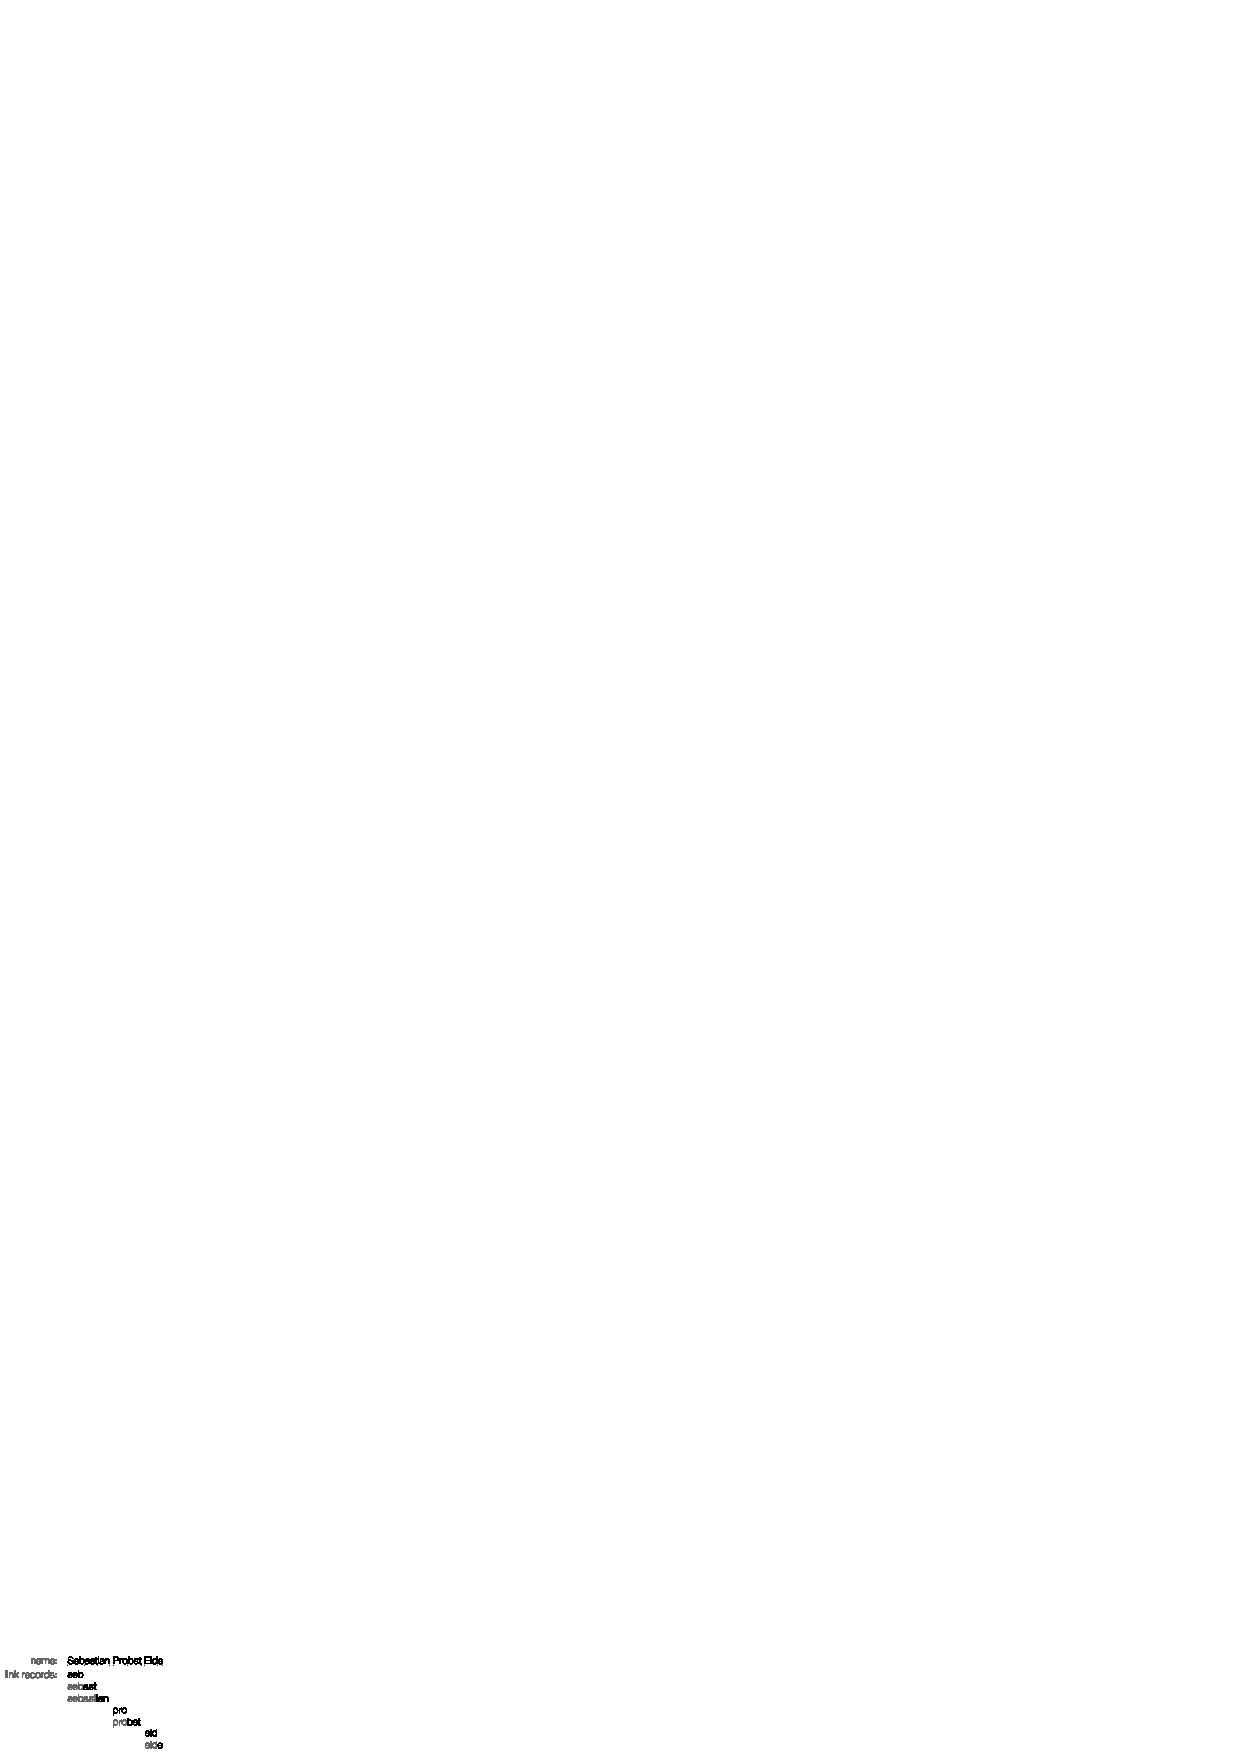
\includegraphics[width=0.6\linewidth]{illustrations/LinkRecords.png}
  \caption{Names are split into name fragments used to generate keys for link records. The slightly darker coloured parts of the link record names indicate the additional three characters added compared to the previous link record name fragment.}
  \label{figLinkRecord}
\end{center}
\end{figure}

When searching for a person the search system looks up \emph{link records} while the user types. Since \emph{link records} contain the full name of the person whose \emph{profile record} they point to, the search system can try to find out which of the possible \emph{profile records} the user is looking for by looking at the relative frequency at which the different \emph{profile records} are being linked to by the \emph{link records} downloaded. It can then download the highest ranked \emph{profile records} and display them as search results to the user while he or she is still completing the search query.

There is an overhead both in terms of storage and lookup cost associated with this approach that I classify and evaluate in the evaluation chapter.

\section{Language and tools used}
%     Learned Erlang
%       Got to know standard libraries and frameworks (OTP)
%       webmachine
%       rebar
%       how to do testing
Wanting to build a highly fault tolerant and distributed system with soft real-time requirements, I decided to use the programming language Erlang.

Erlang, while a language I had never previously used, was created exactly with these requirements in mind. Its standard libraries include frameworks for building hierarchies of process supervisors that ensure processes are restarted if they terminate prematurely or become unresponsive. Erlang also abstracts away inter process communication and encourages immutable state, making problems classical programming languages have with efficient concurrency and shared memory into non-issues.

I learned Erlang and its standard libraries before starting the project, and then selectively read up on more advanced topics as I needed them.

For creating the HTTP based API I used Webmachine, an Erlang framework designed for this purpose. I also used a build tool called rebar.

Testing was done using the built in unit testing framework EUnit, and erlymock was used for testing functions with side effects.

\section{Software engineering practises and planning}
The first basic implementation of my project followed a waterfall approach. Since I spent time up front clarifying  what I wanted my product to do, and had specified the interfaces the components of my system should expose, this allowed me to quickly get a basic version of my system up and running.

Following the initial development cycle, I changed into short iterative bursts where I would adapt and extend the project as I found shortcomings or realized weaknesses in my initial design.

The implementation of the Distributed Hash Tables allowed for a very structured approach. The theory is well understood allowing me to write specifications in the form of tests based on the examples given in the Chord \cite{chord} and Pastry \cite{pastry} papers to ensure my implementations behaved as expected.

I applied test driver practises where I write tests before writing any code for all major parts of the system.

\mbox{}

% Summary:
%   Which steps I took
This chapter analysed what is required for my project to be successful, why an HTTP based API is provided for integration with existing distributed online social networks, and how I proposed a scheme for searching across a key-value store using \emph{link records}.

We also looked at why Erlang was chosen as the language of implementation and also how software engineering practises and planing played a role in the successful implementation of the project.

% Implementation (4000 words)
% * Refer to design strategies that looked ahead to the testing stage
% * Draw attention to what is not my own work (ie rebar, webmachine etc)
% * Major milestones might be highlighted with advantage
% *! Show evidence of skill, clear thinking and common sense

% ************
% Should have: 
% 	intro
% 	content
% 	summary
% ************

% Word budget 4000 words. Try to keep it less
\section{Implementation}

In this chapter I will briefly discuss what data is stored in the Distributed Hash Tables, and also how I get around the problem of efficiently searching through a key-value store and how the changes made to allow this affect the overall performance of the system.

We will then look at what third party libraries are part of the code base, how test-driven development played a crucial part in the development of my project and then go on to look at the high level components that make up the system.

Finally we will discuss how Distributed Hash Tables operate, and more interestingly what distinguishes Chord and Pastry from each other, before we look at how the Erlang concept of process supervision helped me develop a modular and fault tolerant system.

% Content
%   What is to be stored
%     How do we solve search across key's?
%     How much space does this take up?
%       Average name length?
%       Amount of data per user?

\subsection{General discussion}
Before I start discussing how I implemented my project, I want to discuss what data I am interested in storing in my search network, and how I built a search index on top of a distributed hash table. 

\mbox{}

My search network stores records with information about users, much like a normal address book does. I made the following fields mandatory: the person's name, a url to her online social network profile page, and a url to a profile image that can be displayed alongside the search result.

For the purpose of this project I did not want to lock down exactly what data should be stored, but before my system is used in a wider context it would be wise to look into using some well known public standard. At this stage it is outside the scope of my project.

As I briefly discussed in the preparation chapter, a key-value store does not immediately lend itself to search. If you don't know the key under which a data item is stored, you would have to do a linear search across the keyspace in order to find what you are looking for. 

The solution is to use the persons name as the key. Human names in their natural form do not easily map uniformly onto any linear keyspace. They are of different length and also cluster around more common names. I therefore used a hashing function to hash names into keys. This immediately presents us with another problem. If you don't know the exact spelling of the name that was used to generate the key you still can't get around a linear search through the datastore. You can partly solve this problem by normalising names before hashing them into keys, but the utility of a search engine that requires you to already know a complete and correct match of what you are looking for is arguably rather low. Users today increasignly expect search engines to deliver predictive searches where results show before you finish typing your search query. This scheme does neither accommodate this, nor does it misspelled names, or for that matter cases where you have forgotten your friends middle name.

I solved the problem in the following way: Instead of storing just profile records I store both \emph{profile records} and \emph{link records}. The profile records contain all the information stored about a user in the system, and are accessible under a key generated by hashing the whole record. The link records on the other hand are lightweight pointers to the full profile records. They contain the full name and the key of the profile record, and are stored under a key generated by a subset of the users full name. Each profile record has multiple link records pointing to it. I will come back to how I am generating these link records shortly.

Using link records solves several problems. By storing links keyed by fragments of a users name, the search engine can start looking up information before the user has completed typing the search phrase. This enables predictive search. Since the link records also contain the full name of the user you can detect and work around misspelled names, or even searches that don't include all the users names.

% How link records are generated
\begin{figure}[!htb]
\begin{center}
	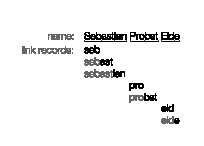
\includegraphics[width=0.6\linewidth]{illustrations/LinkRecords.eps}
  \caption{Here it is shown how a name maps into name fragments used for storing link records pointing to a profile record.}
  \label{figLinkRecord}
\end{center}
\end{figure}

In the current implementation I create link records for each three additional characters contained in a users name. This is illustrated in figure \ref{figLinkRecord}. The process is done separately for each name. Initially the first three characters of a name are taken. Then for the next link records key the subsequent three characters are added. This process is repeated until you reach the end of a name. When you reach the end of a name that is not a multiple of 3, an additional link record is created for the full length of the name. In the example in figure \ref{figLinkRecord} you see this illustrated in how Eide results in the link records \emph{eid} and \emph{eide}.

Using link records does generate extra overhead when searching. A search will now no longer require a single lookup in the search index, but several. As the user types the search server will have to look up link records and resolve them to their profile records. If you searched for my full name, a total of 9 requests would have to be made. 8 for each of the link entries, and an additional one for looking up the full record with all the information about the user. 

In reality it isn't quite as bad as it sounds. The desired result is likely to show up before the user has finished typing, in which case lookups for the remaining link items won't be necessary.

The link items also let the search server rank results by relevance. Let me illustrate this with another example. Say the system contains two profile records: one for Probst and one for Probstonius. If you search for Probst you get two link records, one for \emph{pro} and one for \emph{probst}. Both will return pointers to the profile records of both Probst and Probstonius. Since Probst is a complete match for the search term \emph{probst} while Probstonius is only a partial match, the result for Probst can be given a higher relevance score. The current implementation does this.

The approach of using link records does not come for free. It increases both the amount of data stored per record and also the number of lookups needed in order to find a profile record. I now want to discuss exactly to what extent these parameters are affected.

At my disposal I have a sample of 170 million names from Facebook. While this sample might not entirely accurately reflect all the real names of the human population, I would argue that it closely models the names humans are likely to identify themselves by in online social networks.

By sampling 20 million names and calculating how many link records they would generate, I can say with 99$\%$ confidence that a randomly selected name is likely to generate 5.322 $\pm$ 0.001 link records on average and likewise I can say with 99$\%$ confidence that this particular name will be 14.959 $\pm$ 0.002 characters long on average.
Since each link record consists of a users full name, the key of the profile record and its own key, this will result in roughly 2kbit of extra storage assuming 8 bits per character and 160 bit keys. The benefits of getting predictive searches and the ability to handle misspelled and incomplete names in my opinion greatly outweigh the extra storage requirements.

Estimating how many extra lookups result in using link records is significantly more involved. There will be significant amounts of records sharing the same link records for shorter name segments. If one wants to resolve all of these to their respective profile records, a substantial overhead is incurred. TODO: MAKE SOME EDUCATED GUESSES BASED ON DB of NAMES FROM FACEBOOK and PROJECT COST.

%   Parts not my own
%     Rebar build system
%     Webmachine http arbitrator
%     OTP
%       gen_server
%       supervisors

\subsection{Third party code used}
In this section I want to briefly discuss what third party projects I am using in my project.

Most prominent is my dependence on OTP, the Open Telecom Platform, which is part of the Erlang standard distribution. It is a set of libraries that provide basic functionality needed to write amongst others general servers, and provide functionality for supervising processes within your application and restarting them when they fail. Most Erlang applications rely on OTP.

I also used Webmachine, an open source framework for creating HTTP interfaces in Erlang, and a build system called rebar. Both are developed by Basho.

For testing I used EUnit, part of the standard Erlang distribution, for regular functional unit tests and Erlymock for testing functions with side effects where I wanted to control the functions interactions with the environment.


%   Methology
%     Test driven development
%     Integration testing for gen_server
%   Made it modular.
%   Swappable DHT

\subsection{Process}
At this time it is well understood how Distributed Hash Tables work. The bulk of research in Distributed Hash Tables was done around year 2000. The research papers presenting Chord and Pastry also supply high level code that I referenced when implementing the algorithms. This provided an excellent foundation for doing test-driven development. All the core components of my system were unit tested, and in the tradition of test-driven development I started by writing tests and then wrote the minimal code needed to satisfy my tests. This encourages writing modular systems with self-contained and side effect free functions.
I wrote additional integration tests where I felt it served a purpose.

Modularity was also a key design factor for other reasons. I wanted as many as possible of my modules to be ignorant of which Distributed Hash Table was being used. This encouraged me to keep the interface between the Distributed Hash Tables and the surrounding code strict and minimal. In effect the only methods the Distributed Hash Tables needed to export were ways to get and set values by key.


%   Components of the system
%     Client side
%       Backend
%         Controller
%         DHT's
%       Frontend
%         Search server
%         web api
%       How it all fits together
%     Hub side
%       Web API
%       HubController

\subsection{Components of my system}
I now want to describe the design of my system, and how all the different pieces fit together.

My project has two major parts, each its own application. The search application itself, and a hub application that runs at a central, publicly known location. The hub application acts as a rendevouz point for new Chord and Pastry nodes, and is also used to control and initiate experiments.

\mbox{}

I will first discuss the search application itself:


\subsubsection{The Search application}

% Component overview
\begin{figure}[!htb]
\begin{center}
	\includegraphics[width=0.9\linewidth]{illustrations/ComponentOverview.eps}
\caption{High level overview of the components of the search application. The arrows show how components interact.}
\label{figComponents}
\end{center}
\end{figure}

Figure \ref{figComponents} shows the main high level components of the search system. I will briefly discuss them in turn:

The \emph{Controller} is the heart of the application. It is the point of contact for the central hub application. Through the controller the hub application can choose if the system should run Chord or Pastry nodes, and how many nodes should be run on that particular machine. The controller also issues requests during experimental runs. I will describe this in detail in the evaluation chapter.

The \emph{Distributed Hash Table} component is an arbitrary number of nodes of either of the Distributed Hash Tables Chord and Pastry. Each node has a unique Id and is responsible for part of the keyspace. The nodes are fully autonomous parts of the distributed hash table network.

The \emph{Datastore} is a key-value store responsible for storing the profile and link records. For efficiency reasons the Distributed Hash Tables running on a single machine share the same Datastore. Each record has a \emph{time to live} associated with it. If the record isn't updated before the time to live expires, it is removed from the datastore.

The \emph{Logger} is used during experiments to log the events taking place in the search network. Events can be everything from a node issuing a request, to a request being routed through a node.

The \emph{Friend Search} server is the application actually performing the searches. When a user searches for a name, this name is converted into keys for link records. The search application uses the Distributed Hash Tables to look up the link records and then resolves them to the corresponding profile records that are displayed to the user.
When an online social network wants to make its own profile records searchable, it adds them to its local Friend Search server. The Friend Search server is then responsible for storing the records and corresponding link records in the Distributed Hash Tables and refresh them periodically to ensure they are available in the network.

The \emph{Friend Search Web API} exposes the Friend Search functionality through an HTTP API that can be used by the online social networks to integrate the Friend Search application into their online social networks.

\subsubsection{Hub application}
The hub application is substantially simpler than the search application. It acts as a rendevouz point for new Chord and Pastry nodes to meet in order to join the search network. The hub application also allows me to start and stop Chord and Pastry nodes remotely, as well as start automated experimental runs.

In a real world deployment of my project, the role of the hub application could be limited to simply being a rendevouz point.

\begin{figure}[!htb]
\begin{center}
	\includegraphics[width=0.9\linewidth]{illustrations/HubApp.png}
\caption{The Hub Application interface. A bare-bones web application that allows me to start and stop nodes, change between using Chord and Pastry, and start and stop experiments}
\label{hubApp}
\end{center}
\end{figure}


\subsection{Distributed Hash Tables - 101}
% How DHT's work
% * Quick intro, what will discuss
% *   For each item how Chord and Pastry differ

In this section I will briefly introduce the concept of Distributed Hash Tables. I will then go on to describe how the keyspace is organized and how it is divided amongst nodes participating in a Distributed Hash Table. After that we will look at how Pastry and Chord nodes route messages through their networks.

\mbox{}

% * What is a Dht?
Loosely defined, a Distributed Hash Table is a set of independent entities that have agreed to collectively store and make available a set of data items accessible under keys that fall into a well defined keyspace. Each such entity is generally called a node. 

By design, each node participating in the Distributed Hash Table only needs to know about a subset of the other nodes in the network. By carefully choosing which other nodes a given node knows about, any one node can reach any of the other nodes in a bounded number of hops.
How this is actually done will be discussed shortly.

% * What is the responsibility of a node?
% *   How is keyspace divided up
The keyspace is numeric and ranges from 0, and in the case of my implementations of Chord and Pastry, to $2^{160} - 1$. It wraps around at the boundaries so that 0 is immediately following $2^{160} - 1 $. It can be useful to think of the keyspace as a circle.

Each node is identified by a key. This key is in the same keyspace as the keys for the data stored in the Distributed Hash Table. In one sense nodes are just a special kind of data.

Each node is responsible for a part of the keyspace. All data items with keys in this key segment are stored by that particular node. For this reason it is important that the keys of both the nodes and the data are uniformly spread in the keyspace, so the amount of data stored by any one node is inverse proportional to the number of nodes in the Distributed Hash Table. This in achieved by using strong hash functions. In the case of my implementations I use SHA (FIPS 180-2).

\begin{figure}[!htb]
\begin{center}
	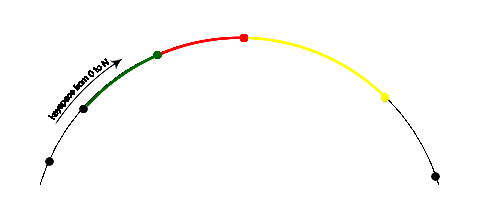
\includegraphics[width=0.9\linewidth]{illustrations/ChordKeySpace.eps}
  \caption{Illustration of how the keyspace is divided between Chord nodes.}
  \label{keyspaceChord}
\end{center}
\end{figure}

\begin{figure}[!htb]
\begin{center}
	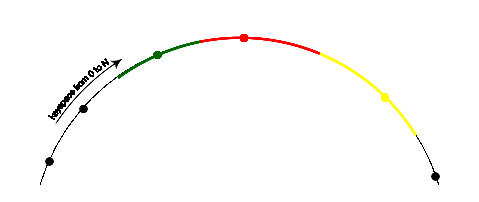
\includegraphics[width=0.9\linewidth]{illustrations/PastryKeySpace.eps}
  \caption{Illustration of how the keyspace is divided between Pastry nodes.}
  \label{keyspacePastry}
\end{center}
\end{figure}

The way in which the subsets of the keyspace is associated with nodes differs slightly between Chord and Pastry. In Chord, a node is responsible for all keys in the range of its predecessors and up to and including itself. In Pastry on the other hand all keys numerically closer to a node than to its neighbour is the responsibility of that particular node. The Chord approach is somewhat easier to implement, but other than that they seem equally well suited for the task.

% * How are the routing tables organized?
% *   What information is stored
% *   How is a message routed from A to B?
% *   How is a key lookup done?

Now that we have discussed how the keyspace is split among nodes in a Distributed Hash Table I will discuss what routing information is required and how messages are actually routed from an origin to a destination. This is the area in which Chord and Pastry differ the most.

\paragraph{The Chord approach to routing}
The Chord routing table is designed in such a way that a node knows many more nodes immediately following it in the keyspace than it does nodes further away. Additionally each node maintains a list of its immediate successors and a pointer to its predecessor in the keyspace.

Whenever a key lookup is performed, the node performing the lookup asks the node in its routing table most closely preceding the target key whether they know about a node closer to the key that still precedes it. If it does, the node performing the lookup in turn asks this node if it knows a closer but preceding node. Once the node immediately preceding the key has been found, its successor is taken as the authority for that particular key.
The data for the key, if present in the network, will be stored by that particular node.
By always asking for the node most closely preceding the target key, we are guaranteed never to overshoot the node responsible for it.

A Chord network works correctly as long as all nodes at all times know who their immediate successor is. If nodes \emph{only} knew about their successor, a key-lookup would necessarily have to do a linear search amongst all the nodes. While this would work it is not efficient. Instead each node maintains a routing table so it has information about nodes further away in the network as well. By design this routing table is such that in a network where all the routing tables are correctly maintained, the number of hops needed are bounded by the logarithm of the number of nodes in the network.


\paragraph{The Pastry approach to routing}
Pastry interprets keys as numbers in some arbitrary base b.
Each node maintains a routing table with an entry per digit in its own key. Each entry represent nodes with keys sharing all the digits up to that particular digits.
When routing a message it is always forwarded to a node that shares \emph{at least} as many digits with the key as the current node does, but additionally is numerically closer to the key. If there is no such node in the routing table, the node checks a table of its immediate neighbours to see if the respective key is in their range. If the given node is the node with a key numerically closest to the message key, the message has arrived at its destination, and is handed over to the Pastry Application.

The number of hops a message has to take is nicely bounded by the parameter b.

\paragraph{Differences between Chord and Pastry}
When constructing and maintaining its routing tables, Pastry uses a proximity heuristic to favour nodes closer to itself. This proximity measure can be anything from latency to the number of routing hops to geographical proximity. Ideally this heuristic should honour the triangle inequality, but in reality this isn't always easy to achieve. In my case I am using the number of routing hops in the actual network topology as a measure. This measure certainly does not honour the triangle inequality, but still seems to offer good performance.

Pastry also maintains a list of nodes that are its neighbours in terms of the proximity metric. These neighbours act as a low cost set of nodes to exchange routing information with.

To what extent these proximity heuristics improve the routing performance will be examined in the evaluation chapter.

\mbox{}

% * Summary
In this section we discussed how the key space is constructed and divided between nodes in Chord and Pastry, and also how Chord and Pastry respectively use their routing tables to route messages to the node responsible for the message key. We also looked at how Pastry uses an additional proximity measure to preferentially route messages through nodes closer to it.

%   How it all fits together

\subsection{Supervision in the context of my project}
In this section I will briefly discuss a key aspect of developing applications in Erlang: The use of supervisors to control application lifetime behaviour.

\begin{figure}[!htb]
\begin{center}
	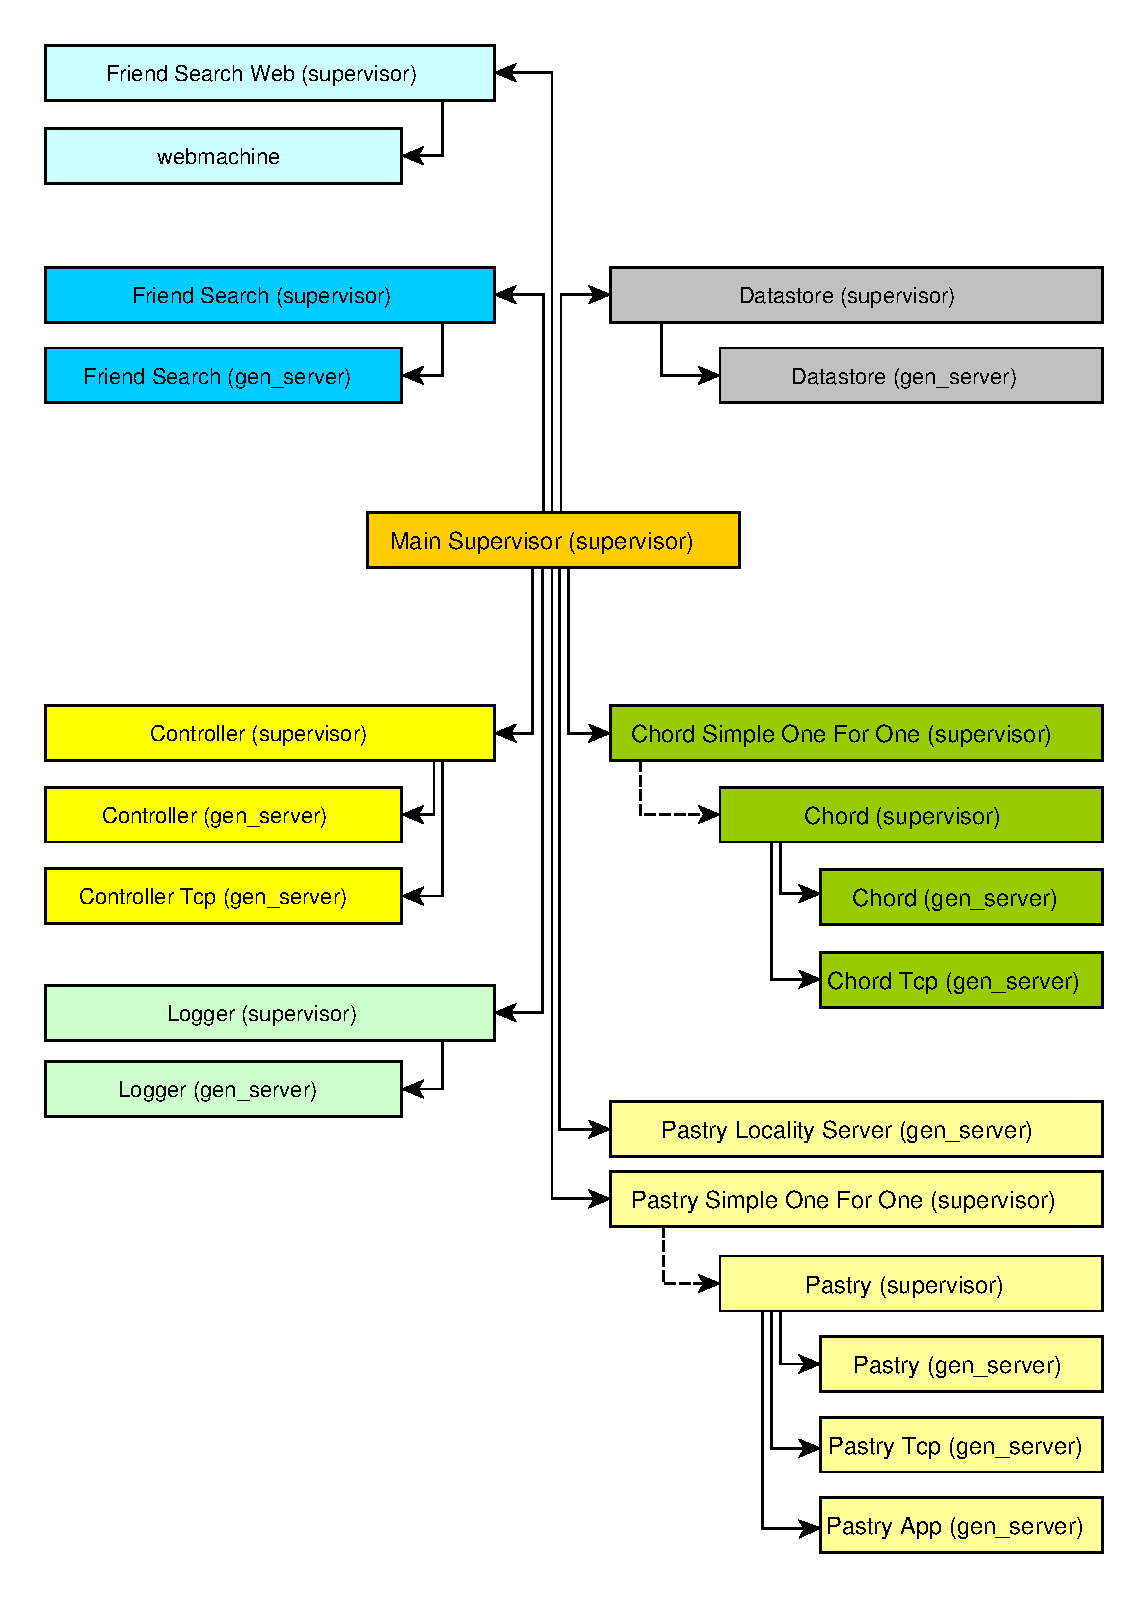
\includegraphics[width=0.9\linewidth]{illustrations/ClientSupervisionTree.eps}
  \caption{This figure shows the same main components as the component diagram shown earlier. It additionally shows the supervisors and gen servers that make up the application.}
  \label{supervisionTree}
\end{center}
\end{figure}

% * The use of supervisors
First let me introduce the concept of supervisors:
Supervisors are processes that are responsible for starting components of an application. For the lifetime of the component they monitor it. If it should fail the supervisor restarts it.

A supervisors supervisees are generally called its children. A supervisor can either have a single child or several children. In the case of supervisors with several children one has to distinguish between supervisors who restart all their children when one fails (one for all), or supervisors only restarting the child that died (one for one). Both types are used in my application. 

I want to introduce one last kind of supervisor that plays a crucial role in my application. It is called a Simple One For One supervisor (simple one for one). A Simple One For One Supervisor specialises in one particular type of children, but has the ability to start and stop arbitrary number of these children at will during the lifetime of the application. This in contrast to regular supervisors who only maintain a predefined set of children. I use this feature to enable the application controller to start and stop Chord and Pastry nodes at runtime.

One last thing we need to know before examining how supervisors are used in my application, is that one can build hierarchies of supervisors.

% * Different types of supervisors
% * What do I use where and why
% * Look at the overall supervision hierarchy of Search Application.
Now let us take a look at the supervision tree of the search application shown in Figure \ref{supervisionTree}.
The main components are the same as in the component overview shown in Figure \ref{figComponents}.

Please take a particularly close look at the Pastry branch of the diagram. The Pastry Simple One For One supervisor only knows about one kind of child: the Pastry Supervisor. The Pastry supervisor in turn knows how to start the main Pastry server component, but also starts the Pastry Tcp component which is the communication component of the Pastry node, and the Pastry Application that is responsible for handling message delivery and storage. The Pastry Supervisor coincidentally is a \emph{one for all} supervisor. When any of its children die, the ones that are alive are also terminated before they are collectively restarted. I decided on this approach as the components are tightly intertwined and rely on a particular instance of the application running.

The Chord branch very much resembles that of Pastry. 

All the other supervisor-child pairs use a \emph{one for one} restart policy.

\mbox{}

We have now seen how supervisors play a crucial part in the design and structure of my project, and how most importantly \emph{simple one for one} supervisors give the flexibility of starting and stopping an arbitrary number of children giving us the flexibility of running an arbitrary number of Chord and Pastry nodes on a single server, and adjusting that number at runtime.

\subsection{Summary of the implementation chapter}
In this chapter we discussed what data is stored in the Distributed Hash Tables, how we got around the difficulties of efficiently searching through a key-value store. We also discussed the negligible additional storage cost of using link records in addition to profile records, and the less negligible overhead of potentially having to resolve a multitude of link records during search.

We looked at what third party libraries have been used, and how test-driven development played a significant role in the development of my project.

We discussed the different main components of the search system, how Chord and Pastry perform key-lookups in their networks and their main differences.

Lastly we also discussed how the Erlang concept of process supervisors plays a role in modularising the code and restarting failing processes.

In the next chapter I will discuss how I evaluated my project and how the performance of Chord and Pastry compare.


% * How many of original goals were achieved? Proved to have been achieved
% * Did the program really work?
% *! Credit for interesting conclusion

% ************
% Should have: 
% 	intro
% 	content
% 	summary
% ************

% What I want to say
%
% Questions to answer:
% * Are Distributed Hash Tables viable data stores for a distributed search engine?
% * Do they scale with size?
% * How do Chord and Pastry compare?
%
% Discuss how started with factorial design with factors of nodes and rate.
% Found doesn't vary over length of run, so any run viable.
% All data from three separate runs.
%
% What looked at was latency and success rate.
% 
% Findings to comment on:
% * Why is Chord so much slower than Pastry?
% * Why does Chord has such a low yield rate compared to Pastry
%
% Conclude
% * Does it work for search engine?

\section{Evaluation}
% TODO: Summarize what I am about to say

\subsection{What to test}
% Questions to answer:
% * Are Distributed Hash Tables viable data stores for a distributed search engine?
% * Do they scale with size?
% * How do Chord and Pastry compare?
% What looked at was latency and success rate.
The approach I will take when evaluation the Distributed Hash Tables Chord and Pastry is quantitative. Their correctness and underlying theory has been widely discussed in research papers and I have nothing new to contribute there. What interests me is if they could work well as data stores in the distributed friend search engine I am proposing to build. To that extent what I will be evaluating is the latency of key lookups, and the success rate of lookups in the network.

We will also look at how they scale with size, and pit Chord against Pastry to see which one performs best.

\subsection{Experimental design}
% Discuss how started with factorial design with factors of nodes and rate.
% Found doesn't vary over length of run, so any run viable.
% All data from three separate runs.
I ran my system on top of machines in the Planet-Lab network. With that in mind, the variables I was able to control where the number of machines participating in the system, the number of Distributed Hash Table nodes running on each machine, and the rate of requests in the network.

In my tests I used all the machines available to me to give some scale to the experiments, and limited the experimental factors to the number of nodes run on each machine and the rate at which requests were issued.

I decided on a factorial design where both node count and rate varied between 1 and 16 in powers of two. For both Chord and Pastry each configuration was run at three different occasions. The three log files combined were then used to give the results I am about to present.

\subsubsection{Experimental pattern}
Each experimental run followed a predefined pattern:
\begin{enumerate}
\item I would ensure that correct number of nodes was running
\item If the number of nodes had to be adjusted, the nodes would be given 3 minutes to update their routing tables.
\item Each machine would clear its previous logs and start its logging machinery.
\item After that the actual experiment would start. Each machine would issue requests to the nodes it hosted at a rate specified for that particular experimental run.
\item After a successfully completed run, there would be a cool down period with continued logging where requests taking slightly longer than permitted would be allowed to finish. Logging would then stop and the logs from the individual machines would be collected at the central hub node.
\item The logs where then downloaded from the central hub to my personal machine for safe keeping and analysis.
\item The process was then repeated for a different set of parameters.
\end{enumerate}

\subsection{Effects of Planet-Lab}
As previously mentioned my experiments ran on top of machines provided by Planet-Lab. I was allowed to run up to 100 machines, but did never manage to get quite that many up and running at the same time.

Using Planet-Lab as a test bed gave me several benefits: the machines at my disposal had a high geographical spread, and varied greatly in what computational resources they provided. Depending on the time of day the computational load on the machines would also vary and not only that, but I would have a different subset of the machines available for testing from day to day.

This infrastructure provided an excellent foundation to test Distributed Hash Tables which are meant to be able to cope with high node churn and machines with widely different capabilities.

While Planet-Lab provides an interesting test bed, its natural variability also makes experiments impossible to accurately repeat. Repeating the same experiment at a different time would invariably give a slightly different result.
To work with Planet-Lab's strengths and not against it, and to at the same time get data I could have confidence in, I ran each experiment repeatedly, shifted in time. This way I ensured I would sample different subsets of the topology. I believe this gives me results that while having higher variance, also more closely resemble the real world scenario Distributed Hash Tables are likely to find themselves in.

\subsubsection{Experimental cleanliness and validity of results}
Performing experiments over longer periods of time showed that the success rate (figure \ref{figLatencyAgainstTime}) and latency (figure \ref{figRateAgainstTime}) stayed constant over time. This allowed me to cut down the length of individual experiments without lowering the quality of my results.

\begin{figure}[!htb]
  \begin{center}
    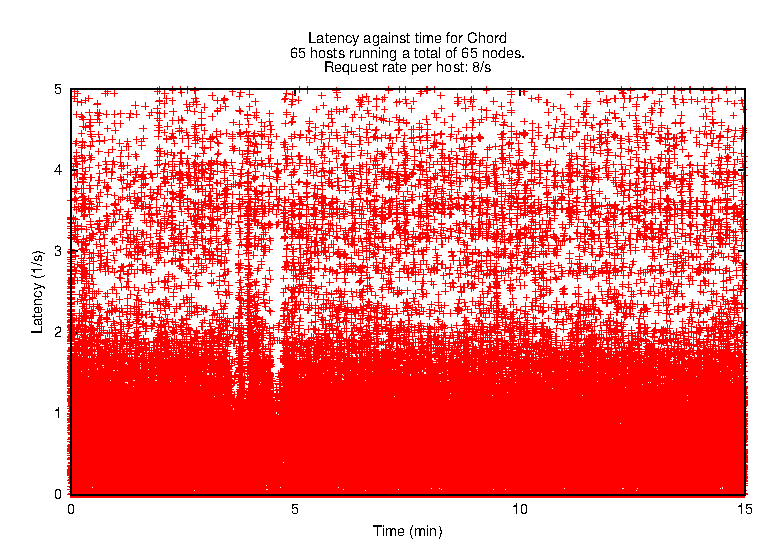
\includegraphics[]{illustrations/latency_aginst_time_chord.eps}
    \caption{This graph shows how latency varies over time in a 15 minute experimental run of Chord.}
    \label{figLatencyAgainstTime}
  \end{center}
\end{figure}

\begin{figure}[!htb]
  \begin{center}
    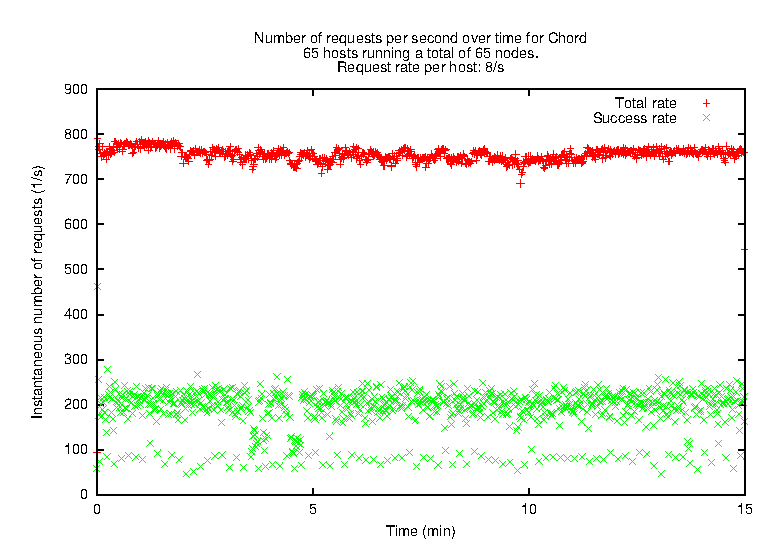
\includegraphics[]{illustrations/rate_against_time_chord.eps}
    \caption{This graph shows how the request rate and success rate varies over a 15 minute experimental run of Chord.}
    \label{figRateAgainstTime}
  \end{center}
\end{figure}

% * How logging not affect results
During experimental runs I would turn of all functionality not directly needed for serving the requests. This would include turning of the mechanisms that kept the nodes routing tables up to date. This initially sounds slightly problematic. If a Distributed Hash Table node disappeared during an experiment, nodes contacting it directly would take note of it, but other nodes wouldn't have the nodes disappearance reflected in their routing state like they would under normal operation. This might seem a somewhat unnatural choice, but makes sense for my experiments for the following reasons:

In my experimental builds of Chord and Pastry I had turned up the rate a which routing information was dissipated through the network to an extreme to make experimental runs shorter. Since what I wanted to test was the raw performance of the system, removing the overhead from keeping the routing tables up to date made sense, especially since this overhead differed between Chord and Pastry, and is a parameter that would have to be tweaked before using this system in any real world deployment.
Also having established that the length of the experimental runs was insignificant made me confident in that not updating routing information during experimental runs did no harm to the experimental results.

% * How load spread evenly
\mbox{}
To ensure even load across my test network, each machine involved individually issued requests to the Distributed Hash Table network.
Keys to access were randomly generated by hashing a combination of the node Id and a time stamp. The result of using this approach is that the keys used for testing differ from experimental run to experimental run. While this makes doing repeatable experiments impossible, it nicely models a real world spread of keys that otherwise would be hard to predict and also evenly spreads the loads between the machines.

% * What constitutes a valid run
Runs where machines vanished during runs would be discarded.


\subsection{Results and comments on results}
Throughout my experiments, a valid request is defined as a request that completes within 5 seconds. By that definition, all other requests are invalid, regardless of if they fail to complete at all, or if they just complete after more than 5 seconds have passed.
% Comment on what is a valid request. And what is considered a failed request
% Findings to comment on:

\subsubsection{Mean latency and success rate for Chord and Pastry}
In figure \ref{figChordLatency} and \ref{figPastryLatency} you see the latency for different rates and different number of nodes per machine for around 60 machines, shown with 95\% confidence intervals. 

What is immediately striking is how much more variance there is in the latencies for Chord than there is in the latencies for Pastry.
In the case of Pastry (figure \ref{figPastryLatency}) we see how the latencies consistently grow for larger number of nodes. Intuitively this is what we would expect as the theory behind the Distributed Hash Tables tells us the number of nodes involved in a look up is proportional to the logarithm of the number of nodes in the network. The same trend is not apparent for Chord (figure \ref{figChordLatency}). On the contrary there is no apparent correlation between the number of notes and the latency for a given rate. What is also peculiar is that, looking at the latencies for a fixed number of nodes per host, the latencies seem to decrease under higher load!

\begin{figure}[htb]
  \centering
  \subfigure[Latency for Chord]{
    \label{figChordLatency}
    \includegraphics[]{illustrations/latency_chord.eps}
  }
  \subfigure[Success rate for Chord]{
    \label{figChordSuccessRate}
    \includegraphics[]{illustrations/success_rate_chord.eps}
  }
  \caption{The graphs above show (a) latencies with 95\% confidence intervals, and (b) success rate for a Chord setup of slightly above 60 nodes.}
\end{figure}

\begin{figure}[htb]
  \centering
  \subfigure[Latency for Pastry]{
    \label{figPastryLatency}
    \includegraphics[]{illustrations/latency_pastry.eps}
  }
  \subfigure[Success rate for Pastry]{
    \label{figPastrySuccessRate}
    \includegraphics[]{illustrations/success_rate_pastry.eps}
  }
  \caption{The graphs above show (a) latencies with 95\% confidence intervals, and (b) success rate for a Pastry setup of slightly above 60 nodes.}
\end{figure}

The success rate Chord (figure \ref{figChordSuccessRate}) and Pastry (\ref{figPastrySuccessRate}) is also dramatically different. Chord seems to perform better when more than one node is run on the same machine, while Pastry's success rate slightly decreases the more nodes are run on the same physical hardware. It is also worth noting that at its best, Chord can't compare with the performance of Pastry.

Unfortunately I have no good explanation for the variations we see within the different configurations for Chord, but I can explain why Chord in the general case performs so much worse than Pastry does and I will do so shortly.

Before that I want to discuss how Chord and Pastry behave when pushed to their limits. The cumulative distribution functions for Chord (figure \ref{figChordCDF}) and Pastry (figure \ref{figPastryCDF}) show the percentage of requests that succeed within five seconds. Each in both cases the experiments are run on roughly 60 machines hosting 1 node each. We see how the success rate in the case of Pastry slowly drops as we get to 128 requests per second per machine.

In the case of Chord on the other hand, the success rate is only marginally worse for 128 and 64 requests per second per hosts than they are when there are 16 requests per second per machine. Also rather odd in the case of Chord is how the rate of 2 per second performs significantly worse than what does the rate of 4. I have no good explanations for this behaviour.

\begin{figure}[htb]
  \centering
  \subfigure[Cumulative distribution function of success against latency for Chord]{
    \label{figChordCDF}
    \includegraphics[]{illustrations/cdf_chord.eps}
  }
  \subfigure[Cumulative distribution function of success against latency for Pastry]{
    \label{figPastryCDF}
    \includegraphics[]{illustrations/cdf_pastry.eps}
  }
  \caption{The graphs above show the cumulative distribution function of a request being successful within the first 5 seconds for (a) Chord, and (b) Pastry.}
\end{figure}

\subsubsection{Why does Chord perform worse that Pastry}
The experimental evidence shown so far clearly shows Pastry as superior to Chord both in terms of latency and in the success rate of requests. I will now try to explain in turn what the cause might be.

\mbox{}

The higher latencies of Chord are the easiest to explain. In figure \ref{figChordNumNodes} and \ref{figPastryNumNodes} you see how many nodes are involved in a particular key lookup in Chord and Pastry respectively. It is clear from the graph that the average number of nodes involved in a key lookup are greater for Chord than for Pastry. If one multiplies the average time it takes to setup a TCP connection with the number of nodes involved, it should be clear that a Chord lookup should take longer if the only thing one is accounting for is the latency of the routing. We are also not factoring in that Pastry uses a heuristic favouring nodes closer by in routing, which additionally should affect the latency as each routing step is likely to take less time than it does for Chord. I will shortly discuss the impact of the proximity heuristic in Pastry.
If the higher number of routing steps for Chord is a bug introduced by me or something inherent to the Chord algorithms is something I can't comment on. It is also possible that the difference would become less significant for larger networks of nodes. Unfortunately this is not something I was able to test given the infrastructure available to me.

\begin{figure}[htb]
  \centering
  \subfigure[Number of nodes involved in key lookup for Chord]{
    \label{figChordNumNodes}
    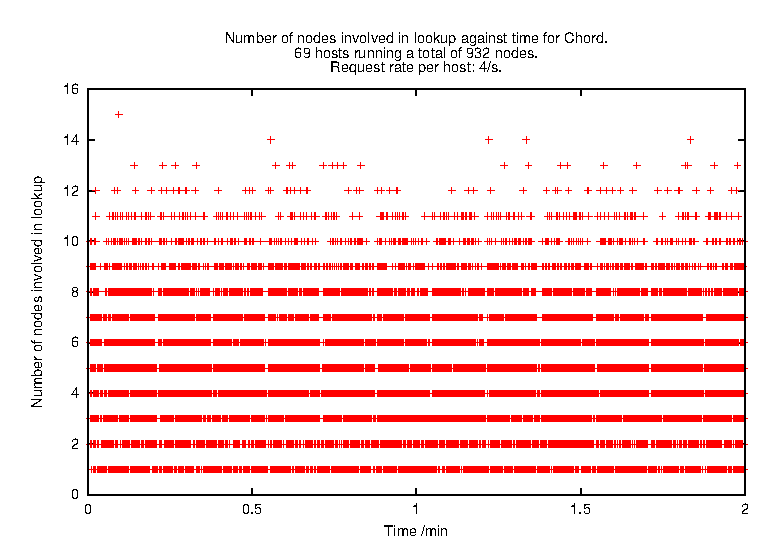
\includegraphics[]{illustrations/nodes_against_time_chord.eps}
  }
  \subfigure[Number of nodes involved in key lookup for Pastry]{
    \label{figPastryNumNodes}
    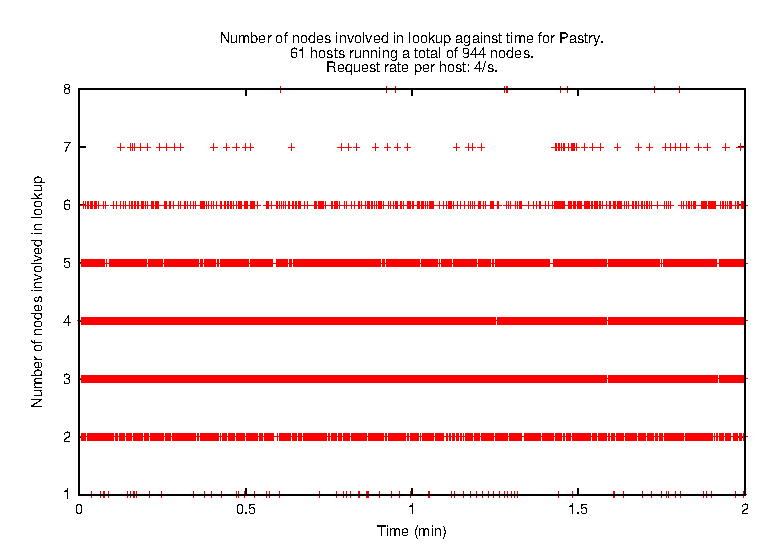
\includegraphics[]{illustrations/nodes_against_time_pastry.eps}
  }
  \caption{The graphs show the number of nodes involved in a key lookup for (a) Chord and (b) Pastry for a particular experimental run.}
\end{figure}

\mbox{}
Now that we have an idea of why the latency might be higher for Chord than for Pastry, let me try to explain why the failure rate might also be higher.

First we let us recall how Chord and Pastry perform their routing.
In Chord, the node that wants to lookup a key (the requester) asks the closest node to the key if they know about other nodes closer to the target key than itself. It then asks the node it gets returned the same question, and the pattern continues until it finds the node preceding the key. Its successor is the target node responsible for the key.

Pastry on the other hand follows a different approach. When a requesting node looks up a key is again makes a request to the node it knows about that is closest to the target node. What differs from the Chord approach though is that the requester hands over the responsibility for the continued lookup to the node it asked. This node in turns then asks another node until the target node has been reached.

Now lets consider what happens when something goes wrong.
In figure \ref{figChordFailedLookup} we see what happens when Chord node A gets returned node D as the next hop node from B. D is not accessible and the lookup fails. If the routing is retried B again returns D, unless it in the meantime itself has noticed that D is inaccessible.

In the Pastry case on the other hand node B becomes responsible for routing the request forward towards the target node. Upon realising node D is unavailable it routes it to the next closest node it knows about, in this case C. Node C happens to know about a closer node to the target than B and this way we managed to route around the dead node D.

There are workarounds to improve the performance of the Chord routing. One would be for the requesting node A to inform node B about node D's death upon retrying to route the message. An alternative could also have been for A to try to route the request through another intermediate node before D, but in this case we are not guaranteed that this intermediate node will not also return D.
A third approach could be to look up D's predecessor, and then use that node in the same role that B filled in this example. None of these methods have been implemented in my implementation as they would extend the core Chord routing algorithm and therefore skew the comparison in Chord's favour.

\begin{figure}[htb]
  \centering
  \subfigure[Failed lookup in Chord]{
    \label{figChordFailedLookup}
    \includegraphics[]{illustrations/ChordRoutingFailed.png}
  }
  \subfigure[Failed lookup in Pastry]{
    \label{figPastryFailedLookip}
    \includegraphics[]{illustrations/PastryRoutingFailed.png}
  }
  \caption{The illustrations show the differences in the routing approach of Chord and Pastry in the case where one of the nodes in the lookup chain is not accessible (Node D). In the case of Pastry it routes around the failed node, while Chord if trying to route again will again get node D returned by node B.}
\end{figure}

% * Why is Chord so much slower than Pastry?
% * Why does Chord has such a low yield rate compared to Pastry
% * How much can we conclude from the numbers?

\subsection{Effect of Pastry routing heuristics}
% * What effect does the Pastry routing heuristics have on the performance
In this section I will try to get a measure to what extent the proximity heuristic used by Pastry affects its routing performance. Be warned that it is rather speculative and relies on some assumptions that cannot necessarily be generalized, but none the less I feel it is interesting food for thought. I will clearly state where I am making assumptions that do not necessarily hold.

The approach I will take is as follows.
This experiment uses a total of 50 nodes. First we look at what overhead is when moving from 50 nodes on 50 different machines to running 5 nodes on each of 10 machines. Since Chord uses no heuristic, we can easily get numbers for how this move affects the routing performance in Chord. In order to relate this Pastry we need a measure for how Pastry and Chord compare when there is no heuristic being used at all. This is rather tricky as the heuristic is tightly integrated into the way Pastry performs its routing. I got this measure by running 50 nodes on a local node on a powerful machine. Since all inter-node communication is on the same machine, the latency is negligible and the routing heuristic plays no part. 

By then comparing the actual impact of moving from 50 machines with one node each to 10 machines with 5 nodes each in the performance of Pastry and comparing the results with what I would have expected them to be, I can estimate how much of an impact the routing heuristic actually had.

The result we get is not necessarily general though, and applying it to random Pastry deployments would be unwise. The results still give an interesting pointer to if such heuristics are beneficial or not.

% TODO: Write shit

I will look at what the overhead is when moving the 100 nodes from 50 separate machines with two nodesfor how much of an impact the Pastry proximity heuristic has on Pastry's routing performance. It is very hard to isolate the effects caused by the heuristic as there are very manywant to quantify to what extent the proximity heuristics used by Pastry increase its performance. 


\subsection{Viability of Distributed Hash Tables a backend store for a search engine}
% Conclude
% * Does it work for search engine?

% TODO: Summary of what we have discussed in this chapter.

% Conclusion (?)
% 	Make it clear in first paragraph what your project was
% 		about and how well you've done it
% 	Will fill in marking sheet after they have done it.
% 	Remind them how awesome project is
% 	If did again, might do... XYZ
% * Refer back to Introduction.
% * How would have planned the project if starting again with benefit of hindsight

% ************
% Should have: 
% 	intro
% 	content
% 	summary
% ************

\section{Conclusion}
In my project I created a search engine to be run by independent and distributed online social networks. The search engine honours the fundamental ideal of independent online social networks of allowing their users control over what and how much data about them is made publicly available, and also solves the problem of allow users of independent online distributed social networks to find and reconnect with their friends regardless of in which online social network they have their profile.

I built this service on top of Distributed Hash Tables and invented a scheme for enabling fuzzy and predictive searches across key-value stores. This scheme works well in its current form for installations with small to medium sized data sets, and could work well in larger installations if slightly tweaked.

As part of my project I implemented two Distributed Hash Tables. While both work correctly, my implementation of Pastry works significantly better than Chord, and gives quite impressive results.

My project was highly successful as a proof of concept, but would need further refinement before being deployed by real social networks, which is in line with what I set out to do. 

\mbox{}

While being a success in its own right, the project has also been an excellent learning experience.
I had never used the programming language Erlang for anything but trivial ``hello world" applications before the start of my project and now have a solid working knowledge of it and its libraries. I also got significant exposure to working with highly distributed systems and deploying software across up to 100 machines.
The same project implemented again from the beginning would cost me significantly less time and effort considering all the knowledge I now possess, but that itself can also be considered a success, considering knowledge acquisition is a central component of what role I believe the Part 2 projects are designed to achieve.

\mbox{}

As a whole the project solves a very real problem that needed addressing to help independent distributed social networks stand a fighting chance in gaining ground against the social network gorilla Facebook. There is still a lot of work that needs doing, but my project serves an important role in highlighting an important obstacle that needs addressing and proposed a solution for how it can be tackled.

\addcontentsline{toc}{chapter}{Bibliography}
\begin{thebibliography}{9}

\bibitem{progerlang}
  Joe Armstrong,
  \emph{Programming Erlang, Software for a Concurrent World}.
  The Pragmatic Programmers,
  Version: 2008-7-6.

\bibitem{erlangprog}
  Francesco Cesarini and Simon Thompson,
  \emph{Erlang programming}.
  O'Reilly Media,
  2009.

\bibitem{chord}
  Ion Stoica, Robert Morris, David Karger, M. Frans Kaashoek, Hari Balakrishnan,
  \emph{Chord: A Scalable Peer-to-peer Lookup Service for Internet Applications}.
  MIT Laboratory for Computer Science.

\bibitem{pastry}
  Antony Rowstron	and Peter Druschel,
  \emph{Pastry: Scalable, decentralized object location and routing for large-scale peer-to-peer systems}.
  Microsoft Research Ltd, St. George House.

\bibitem{kademila}
  Peter Maymounkov and David Mazieres,
  \emph{Kademilia: A Peer-to-peer Information System Based on the XOR Metric}.
  New York University.

\bibitem{tapestry}
  Ben Y. Zhao, Ling Huang, Jeremy Stribling, Sean C. Rhea, Anthony D. Joseph, Member, IEEE, and John D. Kubiatowicz, Member, IEEE,
  \emph{Tapestry: A Resilient Global-Scale Overlay for Service Deployment}.

\bibitem{dht}
  \emph{Wikipedia: Distributed Hash Tables}.
  http://en.wikipedia.org/wiki/Distributed\_hash\_table.
  
\bibitem{experimental_design}
  Dr David Evans
  \emph{Lecture notes on Experimental Design}.
  CS 457/657,	Winter 2005.

\bibitem{tcp}
  Serge Aleynikov,
  \emph{Building a Non-blocking TCP server using OTP principle}.
  TrapExit.org / http://www.trapexit.org/Building\_a\_Non-blocking\_TCP\_server\_using\_OTP\_principles.

\bibitem{gen_tcp}
  Andreas Stenius,
  \emph{gen\_listener\_tcp}.
  Github.org / https://github.com/kaos/gen\_listener\_tcp.

\bibitem{erlymock}
  Jason Wagner,
  \emph{erlymock}.
  Github.org / https://github.com/nialscorva/erlymock/wiki.

\bibitem{erlangtdd}
  Jason Wagner,
  \emph{Erlang, Testing and TDD}.
  http://erlcode.wordpress.com/.

\bibitem{webmachine}
  Basho,
  \emph{Webmachine documentation}.
  http://webmachine.basho.com/.

\end{thebibliography}

\chapter{Routing state as Erlang data structures}
\label{sec:appendixErlangRoutingState}
I use Erlang records for the Chord and Pastry routing state.
When regular tuples are used to pass data-structures between functions, the amount of code that needs updating when the data structure evolves is often substantial.
While you need to write out the full structure of a tuple to pattern match on one of its values, records give you direct access to named members of the structure, abstracting away the physical layout of the data.
Under the hood, records are still compiled down to regular tuples, but this is handled transparently  without the programmer needing to know about it or update code where the data-structure is being used.

\section{Chord routing state}
Code listing \ref{listingChordDataStructures} shows how I translated the Chord routing state described in section \ref{sec:chordRoutingState} on page \pageref{sec:chordRoutingState} into Erlang records.

\lstinputlisting[label=listingChordDataStructures,caption=Chord routing table as Erlang records]{sourceCode/chord_routing_table.erl}

\section{Pastry routing state}
Code listing \ref{listingPastryDataStructures} shows how I translated the Pastry routing state described in section \ref{sec:pastryRoutingState} on page \pageref{sec:pastryRoutingState} into Erlang records.
The distance field on line 6 in the node record in the listing is the numeric distance between a particular node and the node maintaining the routing state, as returned by the proximity heuristic used for routing.

\lstinputlisting[label=listingPastryDataStructures,caption=Pastry routing table as Erlang records]{sourceCode/pastry_routing_table.erl}

%-----------------------------------------------------------
% Pastry Erlang Routing
%-----------------------------------------------------------
\chapter{Pastry routing algorithm in Erlang}
\label{sec:appendixErlangRoutingAlgorithm}
This section compliments section \ref{sec:routingInPastry} on page \pageref{sec:routingInPastry} and shows how I translated the Pastry pseudo code routing algorithm into Erlang.

\mbox{}

My Erlang implementation of the Pastry routing algorithm, rather than being a direct translation of the pseudo code (listing \ref{listingPastryPseudocode} on page \pageref{listingPastryPseudocode}), takes the essence of what the Pastry routing algorithm tries to accomplish, and implements that.

The code in listing \ref{listingRouteMsg} shows my main Erlang \verb=route_msg= function. 
Just like the pseudo code in pseudo code listing \ref{listingPastryPseudocode} on page \pageref{listingPastryPseudocode} it tries routing via the leaf set, then the routing table and if all else fails to any node that is closer to the target key.

\lstinputlisting[label=listingRouteMsg,caption=Routes a message towards a recipient]{sourceCode/route_msg.erl}

In listing \ref{listingRouteToLeafSet} we see that if the match in the leaf set is the node itself, then on line 5 the message is delivered to the main pastry application. Otherwise the message is forwarded to a closer node if appropriate on line 7.

\lstinputlisting[label=listingRouteToLeafSet,caption=Routes a message to the leaf set if applicable]{sourceCode/route_to_leaf_set.erl}

If routing to the leaf set fails (line 3 in listing \ref{listingRouteToLeafSet}), the node tries routing the message to a node in the routing table sharing more digits in the key with the message key than what itself does. Again, just like when routing to the leaf set, if the best match is itself, the message is delivered. This function is shown in code listing \ref{listingRouteToNodeInRoutingTable}.

It is not quite as easy to see how this code listing corresponds to the pseudo code in listing \ref{listingPastryPseudocode} on page \pageref{listingPastryPseudocode}. For example, in the listing \ref{listingRouteToNodeInRoutingTable} there is nothing that directly correspond to getting the length of the shared key path as we see on line 9 in the Pastry pseudo code in listing \ref{listingPastryPseudocode} on page \pageref{listingPastryPseudocode}. Instead what the Erlang implementation does is find all the nodes in the routing table that share as many key digits with the message key as the node itself does (line 2) in addition to the \verb=PreferredKeyMatch= (also line 2) which is the shared key-segment plus the first digit in the message key that differs from the key of the node itself.
On line 4 we look for a node in the list of nodes which shares all the digits in the \verb=PreferredKeyMatch=. If there is one then the message is passed on to that node and if there is none, we return empty handed.

\lstinputlisting[label=listingRouteToNodeInRoutingTable,caption=Routes a message to a node in the routing table]{sourceCode/route_to_node_in_routing_table.erl}

If all other routing approaches fail, the last resort the Pastry node has is to find any node that is numerically closer to the key than what itself is. Code listing \ref{listingRouteToCloserNode} shows the Erlang implementation finding the key segment shared between the message key and the node's key (line 2) and then finding all the nodes it knows about that share this key segment (line 3). On line 7 the node numerically closest to the message key is found and the message either forwarded or delivered.

\lstinputlisting[label=listingRouteToCloserNode,caption=Routes a message to any closer node]{sourceCode/route_to_closer_node.erl}

%---------------------------------------
% Link record optimizations
%---------------------------------------

\chapter{Optimizing the link records approach}
\label{sec:appendixLinkRecords}
This appendix on optimizing the link record approach to search compliments section \ref{sec:costOfLinkRecords} on page \pageref{sec:costOfLinkRecords} where I discuss the cost of using link records to enable predictive and fuzzy searches on top of Distributed Hash Tables.

\mbox{}

An optimization that could be quite promising, but is not part of my current search server implementation, is to not start looking for link records unless the search term exceeds a minimum length.
The immediate drawback of this approach is that it is less interactive, but this lack of interactivity could easily be camouflaged by having the search engine display matches taken from data cached from local caches resulting from previous searches, and adaptively load more results from the distributed search network as the query gets longer.
The threshold has to be matched to the way the link records are generated. Say if we generated link records for each additional 5 characters and had set the threshold to 4, then no correct matches could ever be found for names longer than 5 characters before the 5th character in the search query has been entered. That is unless cached results already exist on the search engine node.
The threshold value has to be set according to how long the average name is. There are a significant proportion of names 4 character or less in length, and by setting the threshold to a value higher than 4 these short names would never be found using the predictive search unless they had already been cached.
One would also have to consider if the threshold should be a per name threshold, by which I mean that we do not look up link records for name fragments shorter than the threshold, or a per query threshold, in which case surnames would already trigger a link record lookup after their first character has been entered, which in the case of the letters \emph{a} and \emph{b} would trigger 47 and 21 MB downloads of link records respectively (from table \ref{tableIndianName} on page \pageref{tableIndianName} and \ref{tableAmericanName} on page \pageref{tableAmericanName} respectively). It could be a good idea to set the threshold on a per name basis, but continue to order and prioritize the already downloaded link records given the full name component they contain already from the very first character the user types in the subsequent names.
I believe setting a search threshold of 2 or 3 characters combined with generating link records for each additional 4 characters could be a good compromise. It would allow us to find the short names interactively, and would still ensure a relative sparsity of link records.

The danger with generating link records for too long name fragments is that it makes fuzzy searching harder to achieve, as fuzzy searches rely on either already having found the correct link record before the spelling mistake is done, or find a correct link record for one of the person's other names and then give that a higher priority due to it being a close match for the misspelled full name.

\mbox{}

Another optimisation to the link record worth considering is how one could compress the data they occupy in the search network and that needs to be transferred during search.
In the current implementation link records quite unnecessarily store their own key. 160-bit keys also take up 192 bits of spate on 64-bit machines and the names themselves are not at all compressed.
If one removed the self-referencing keys, used 128-bit keys and compressed the full name by a factor of 2, then a link record could take 125 bytes instead of 300 bytes per record, which would reduce the storage and transfer requirements by a factor of 2.4. 

%---------------------------------------
% Source code
%---------------------------------------

\chapter{Source code}
My project is fully open sourced. The source code can be found on my github account under: https://github.com/sebastian/Part-2-project

% Below follows the source code listing of the Pastry core implementations.
% Tests are not included.
% 
% The full project source code can be found on github: https://github.com/sebastian/Part-2-project
% 
% \lstinputlisting[label=pastry_implementation,caption=Implementation of Pastry]{sourceCode/pastry.erl}

Index coming here if needed... Think I'll skip it


\cleardoublepage

% Draft #1 (final?)

\vfil

\centerline{\Large Friend search for distributed social networks }
\vspace{0.4in}
\centerline{\large Sebastian Probst Eide, St Edmunds College }
\vspace{0.3in}
\centerline{\large Originator: Sebastian Probst Eide}
\vspace{0.3in}
\centerline{\large 4 October 2010}

\vfil

\subsection*{Special Resources Required}
Personal laptop for development and initial testing (1.86 Ghz, 2GB Ram) \\
CL machine with the Erlang VM installed as a backup \\
Virtual Server infrastructure, the like of Amazon EC2, for parts of the evaluation \\
\vspace{0.2in}

\noindent
{\bf Project Supervisors:} Dr David Eyers and Dr David Evans
\vspace{0.2in}

\noindent
{\bf Director of Studies:} Dr Robert Harle
\vspace{0.2in}
\noindent
 
\noindent
{\bf Project Overseers:} Unknown ********** PLEASE UPDATE! ***********

\vfil
\pagebreak

% Main document

\section*{Introduction}

It is hard to get started using independent, distributed online social networks as it is frequently difficult to find and connect with your existing friends, not knowing in which social networking system(s) they host their profiles and where those networks are hosted. The purpose of this project is to lay the foundation for a decentralised and distributed friend search engine that can be offered alongside installations of independent social networks allowing users to easily reconstruct their social graph in the online social network(s) of their choice. The focus of the project will be on the data storage layer of the search engine. I will compare and contrast different Distributed Hash Tables that I implement in Erlang. Erlang is chosen because it is known to be well suited for developing concurrent and distributed systems.

A front end, allowing basic searches to be performed, will also be created, but mainly to provide a way to rapidly exercise the data storage layer. More user-oriented functionality needed to allow the project to be used on a larger scale will be left out so as to limit the scope of the project.

\section*{Work that has to be done}

There are a number of distributed hash table designs available.\footnote{ Wikipedia currently lists 8 different protocols } I have decided to implement and compare the following three, chosen because they are well documented algorithms but importantly differ in the way they perform their routing: Chord, Kademilia and Pastry. As an example in how they differ, consider how Pastry allows for heuristics based on anything from ping to available bandwidth or combinations thereof, Kademilia uses XOR arithmetic to determine the distance between nodes as a routing heuristic, while Chord has none of the above, using simplicity as its strength. These different approaches to the same problem make the algorithms excellent candidates to compare.

The main parts of the project are to:

\begin{itemize}
  \item Implement the data storage layer of the search engine in Chord, Kademilia and Pastry using a uniform API that allows the system to use any one of the three without additional changes
  
  \item Implement infrastructure that facilitates testing and monitoring of the system. More specifically it should allow:

  \begin{itemize}
    \item Starting and stopping virtual servers across the different service providers to minimize server rental costs between testing sessions. The servers will be used to test different aspects of the distributed hash tables
    \item Start and stop search nodes across the physical servers
    \item Display how many search nodes are available in the system, and potentially some metric for how they are interconnected in terms of latency and bandwidth
    \item Add and remove test data from the system. The system will be tested with \emph{Database of names} from Facebook which I have access to. It is of significant size and importantly, contain keys with non-random distributions making for a more realistic dataset
    \item Perform repeatable load testing on the system where tests as an example could compare read/write performance for different key and value sizes and different numbers of key-value pairs
    \item Count the number of jumps and the time a key lookup needs in order to find a data item, in addition other appropriate descriptive statistical measures for writes and lookups in fixed key-value datasets
    \item Being able to eliminate and add subsets of storage nodes in a repeatable fashion to test how the different Distributed Hash Tables cope with nodes disappearing and appearing
  \end{itemize}

  \item Setup a Linux image that can be run across Infrastructure as a Service providers\footnote{Vagrant seems like a likely candidate to help automate this (http://vagrantup.com)}

  \item Implement a web front end to allow users to perform basic searches across the data storage layer

\end{itemize}

Please note that while the following aspects of the search server are secondary to the project and will not initially be implemented, they all, should time permit, serve as excellent project extensions:

\begin{itemize}
  \item Fuzzy searches allowing the user to misspell names. 
  \item Support composite keys to allow searching for different attributes of a record
  \item Predictive searches
  \item Searches taking knowledge about social circles from online social networks, or similar metadata, into account in order to more intelligently prioritise and order the search results returned to the user
  \item Protections against malicious use of the storage network like broadcasting data, attempting to overload nodes with requests or using the network to store spam or pollute the namespace with spammy records
\end{itemize}


\section*{Starting Point}

I have a reasonable working knowledge of Erlang and Linux and development of web based systems. The algorithms that will be implemented have all previously been implemented in other languages, and are used in production systems, so finding information about them should be possible. I have not yet used Amazon EC2 or any of the other Infrastructure as a Service (IaaS) providers that could be used to perform testing on the system in a distributed manner.


\section*{Success criterion}

I regard the project as successful if I have working implementations of the three Distributed Hash Tables that allow me to set and retrieve values based on keys across a distributed network of machines, and also metrics for how the performance of key-lookup varies by node-, key-count and distributed hash table type and recommendations for future work based on the metrics collected.

The search component of the project, which is the application part that uses the distributed hash tables as a datastore to allow users to find their friends, has been left out of the success criterion due to it being harder to quantify and evaluate well.

\section*{Difficulties to Overcome}

The following main learning tasks will have to be undertaken before 
the project can be started:

\begin{itemize}

\item To learn and fully understand the Chord, Kademilia and Pastry algorithms.

\item To learn how to do network communication in Erlang other than the built in message passing. I prefer the individual nodes to communicate over TCP or UDP as that frees the design from assumptions regarding the language of implementation, and also removes the substantial overhead incurred by having each Erlang VM keep track of the state and availability of all the other nodes network wide, which would be in stark contrast with the distributed hash tables need to only maintain rather minimalistic routing tables. Additionally there are security issues when allowing Erlang VMs to connect directly in untrusted networks as any node is allowed to execute arbitrary code on any other connected node

\item To find a way to test the system on geographically distributed nodes.

\end{itemize}


\section*{Resources}

Some aspects of this project (amongst others the heuristics in Pastry that take locality into account when routing) are more interesting to test in nodes that are geographically distributed. For this reason using server instances from a provider like Amazon AWS or PlanetLab seem like a good idea. Ways of getting access to time on such infrastructure for academic purposes is currently being looked into. For the majority of the development cycle local testing will be just as interesting and can be done on my development machine.

This project requires no additional file space on University machines. I will be hosting the project source code and dissertation files in a repository on github.\footnote{http://github.com/sebastian/Part-2-project}
If my machine breaks down, the development can be continued on any Unix based machine that has VIM, git and the Erlang VM installed.

\section*{Work Plan}

Planned starting date is 15/10/2010. 

Below follows a list of tasks that need to be done:

\begin{itemize}
  \item Work through the theory behind Chord, Kademilia and Pastry and other items listed under \emph{difficulties to overcome} (2 weeks).
  \item Implement initial version of Chord, Kademilia and Pastry in Erlang (4 weeks)
  \item Implement test harness to perform testing of the system (4 weeks)
  \item Implement a web frontend for search alongside a search server written in Erlang, that uses the distributed data storage layer for its data (2 weeks).
  \item Write dissertation (6 weeks).
\end{itemize}

\subsection*{Michaelmas Term} 

By the end of this term I intend to have completed the research and learning tasks and have finished the first implementations of the Distributed Hash Tables in Erlang. In the vacation that follows I intend to make a good start on the testing harness and do a little work on the search server.


\subsection*{Lent Term}

In the first half of this term I intend to finish the test harness and search server and spend time testing the system and solving problems. The tests could follow a factorial design where distributed hash table type, number of nodes, key-size, payload size, number of entries in the system and geographical distribution are all factors worth considering. What levels should be considered for each factor is yet to be determined and will become clearer as the project develops.

In the second half of this term I tend to get an initial draft of my dissertation written.


\subsection*{Easter Term}

In this term I plan to polish the dissertation. The estimated completion date is the 15th of May, leaving a couple of days to let the dissertation rest before giving it a final read and correcting last minute mistakes before the due date on the 20th of May.


\end{document}
